\documentclass[12pt]{article}
\usepackage[margin=2.5cm]{geometry}
\usepackage{enumerate}
\usepackage{amsfonts}
\usepackage{amsmath}
\usepackage{fancyhdr}
\usepackage{amsmath}
\usepackage{amssymb}
\usepackage{amsthm}
\usepackage{mdframed}
\usepackage{graphicx}
\usepackage{subcaption}
\usepackage{soul}
\usepackage[utf]{kotex}

\begin{document}
\title{Worksheet 20 Solution}
\author{Hyungmo Gu}
\maketitle

\section*{Question 1}
\begin{enumerate}[a.]
    \item

    \bigskip

    \begin{proof}

    Let $V = \{1,2,3,4,5,6\}$, $E = \{(1,2),(1,6),(2,3),(3,4),(4,5),(5,6)\})$.

    \bigskip

    We need to prove the graph $G = (V,E)$ is bipartite by proving the following
    properties:

    \begin{enumerate}[1.]
        \item There exists subsets $V_1, V_2 \subset V$ such that
        $V_1 \neq \emptyset, V_2 \neq \emptyset$, and $V_1$ and $V_2$ form
        a partition of $V$.
        \item Every edge in $E$ has exactly one endpoint in $V_1$ and one in $V_2$.
    \end{enumerate}

    \bigskip

    We will prove the properties in parts.

    \bigskip

    \ul{\textbf{Part 1 (Proving $V_1 \neq \emptyset, V_2 \neq \emptyset$,
    and $V_1$ and $V_2$ form a partition of $V$):}}

    \bigskip

    Let $V_1 = \{1,3,5\}$ and $V_2 = \{2,4,6\}$.

    \bigskip

    We need to prove $V_1 \neq \emptyset, V_2 \neq \emptyset$, and
    $V_1$ and $V_2$ form a partition of $V$, i.e $V_1 \cup V_2 = V
    \land V_1 \cap V_2 = \emptyset$.

    \bigskip

    First, we need to show the subsets $V_1$ and $V_2$ are non-empty.

    \bigskip

    The header tells us both subsets $V_1$ and $V_2$ have more than
    1 elements.

    \bigskip

    Then, using these facts, we can conclude $V_1 \neq \emptyset$ and
    $V_2 \neq \emptyset$.

    \bigskip

    Finally, we need to show $V_1 \cup V_2 = V$ and $V_1 \cap V_2 = \emptyset$.

    \bigskip

    The header tells us $V_1 = \{1,3,5\}$ and $V_2 = \{2,4,6\}$.

    \bigskip

    Then, we can calculate

    \begin{align}
        V_1 \cup V_2 &= \{1,2,3,4,5,6\} = V\\
        V_1 \cap V_2 &= \emptyset
    \end{align}

    \bigskip

    \ul{\textbf{Part 2 (Proving every edge in $E$ has exactly one endpoint
    in $V_1$ and\\ one in $V_2$):}}

    \bigskip

    Let $V_1 = \{1,3,5\}$ and $V_2 = \{2,4,6\}$.

    \bigskip

    We need to show every edge in $E$ has exactly one endpoint in $V_1$ and
    one in $V_2$.

    \bigskip

    The header tells us $V_1 = \{1,3,5\}$, $V_2 = \{2,4,6\}$,
    and $E = \{(1,2),(1,6),(2,3),\\(3,4),(4,5),(5,6)\})$.

    \bigskip

    Using these facts, we can generate the following table.

    \bigskip

    \begin{tabular}{|c|p{3cm}|c|p{3cm}|}
        \hline
        Edge (1,2) & - 1 is in $V_1$ \newline - 2 is in $V_2$ & Edge (3,4) & - 3 is in $V_1$ \newline - 4 is in $V_2$\\
        \hline
        Edge (1,6) & - 1 is in $V_1$ \newline - 6 is in $V_2$ & Edge (4,5) & - 4 is in $V_2$ \newline - 6 is in $V_1$\\
        \hline
        Edge (2,3) & - 2 is in $V_2$ \newline - 3 is in $V_1$ & Edge (5,6) & - 5 is in $V_1$ \newline - 6 is in $V_2$\\
        \hline
    \end{tabular}

    \bigskip

    Then, it follows from observation that every edge in $E$ has
    one endpoint in $V_1$ and one in $V_2$.

    \end{proof}

    \bigskip

    \begin{mdframed}
        \underline{\textbf{Pseudoproof:}}

        \bigskip

        Let $V = \{1,2,3,4,5,6\}$, $E = \{(1,2),(1,6),(2,3),(3,4),(4,5),(5,6)\})$.

        \bigskip

        We need to prove the graph $G = (V,E)$ is bipartite by proving the following
        properties:

        \begin{enumerate}[1.]
            \item There exists subsets $V_1, V_2 \subset V$ such that
            $V_1 \neq \emptyset, V_2 \neq \emptyset$, and $V_1$ and $V_2$ form
            a partition of $V$.
            \item Every edge in $E$ has exactly one endpoint in $V_1$ and one in $V_2$.
        \end{enumerate}

        \bigskip

        We will prove the properties in parts.

        \bigskip

        \begin{enumerate}[1.]
            \item Show there exists subsets $V_1, V_2 \subset V$ such that
            $V_1 \neq \emptyset, V_2 \neq \emptyset$, and $V_1$ and $V_2$ form
            a partition of $V$

            \bigskip

            Let $V_1 = \{1,3,5\}$ and $V_2 = \{2,4,6\}$.

            \bigskip

            We need to prove $V_1 \neq \emptyset, V_2 \neq \emptyset$, and
            $V_1$ and $V_2$ form a partition of $V$, i.e $V_1 \cup V_2 = V
            \land V_1 \cap V_2 = \emptyset$.

            \bigskip

            \begin{enumerate}[1.]
                \item Show $V_1 \neq \emptyset, V_2 \neq \emptyset$

                First, we need to show the subsets $V_1$ and $V_2$ are non-empty.

                \begin{mdframed}
                The header tells us both subsets $V_1$ and $V_2$ have more than
                1 elements.

                \bigskip

                Then, using these facts, we can conclude $V_1 \neq \emptyset$ and
                $V_2 \neq \emptyset$.

                \end{mdframed}

                \item Show $V_1 \cup V_2 = V \land V_1 \cap V_2 = \emptyset$

                \bigskip

                Second, we need to show $V_1 \cup V_2 = V$ and $V_1 \cap V_2 = \emptyset$.

                \bigskip

                \begin{mdframed}
                The header tells us $V_1 = \{1,3,5\}$ and $V_2 = \{2,4,6\}$.

                \bigskip

                Then, we can calculate

                \begin{align}
                    V_1 \cup V_2 &= \{1,2,3,4,5,6\} = V\\
                    V_1 \cap V_2 &= \emptyset
                \end{align}

                \end{mdframed}

            \end{enumerate}

            \bigskip

            \begin{mdframed}
            \underline{\textbf{Part 1:}}

            \bigskip

            Let $V_1 = \{1,3,5\}$ and $V_2 = \{2,4,6\}$.

            \bigskip

            We need to prove $V_1 \neq \emptyset, V_2 \neq \emptyset$, and
            $V_1$ and $V_2$ form a partition of $V$, i.e $V_1 \cup V_2 = V
            \land V_1 \cap V_2 = \emptyset$.

            \bigskip

            First, we need to show the subsets $V_1$ and $V_2$ are non-empty.

            \bigskip

            The header tells us both subsets $V_1$ and $V_2$ have more than
            1 elements.

            \bigskip

            Then, using these facts, we can conclude $V_1 \neq \emptyset$ and
            $V_2 \neq \emptyset$.

            \bigskip

            Finally, we need to show $V_1 \cup V_2 = V$ and $V_1 \cap V_2 = \emptyset$.

            \bigskip

            The header tells us $V_1 = \{1,3,5\}$ and $V_2 = \{2,4,6\}$.

            \bigskip

            Then, we can calculate

            \begin{align}
                V_1 \cup V_2 &= \{1,2,3,4,5,6\} = V\\
                V_1 \cap V_2 &= \emptyset
            \end{align}
            \end{mdframed}

            \item Show every edge in $E$ has exactly one endpoint in $V_1$ and one in $V_2$.

            \bigskip

            Let $V_1 = \{1,3,5\}$ and $V_2 = \{2,4,6\}$.

            \bigskip

            We need to show every edge in $E$ has exactly one endpoint in $V_1$ and
            one in $V_2$.

            \bigskip

            \begin{mdframed}

            The header tells us $V_1 = \{1,3,5\}$, $V_2 = \{2,4,6\}$,
            and $E = \{(1,2),(1,6),(2,3),\\(3,4),(4,5),(5,6)\})$.

            \bigskip

            Using these facts, we can generate the following table.

            \bigskip

            \begin{tabular}{|c|p{3cm}|c|p{3cm}|}
                \hline
                Edge (1,2) & - 1 is in $V_1$ \newline - 2 is in $V_2$ & Edge (3,4) & - 3 is in $V_1$ \newline - 4 is in $V_2$\\
                \hline
                Edge (1,6) & - 1 is in $V_1$ \newline - 6 is in $V_2$ & Edge (4,5) & - 4 is in $V_2$ \newline - 6 is in $V_1$\\
                \hline
                Edge (2,3) & - 2 is in $V_2$ \newline - 3 is in $V_1$ & Edge (5,6) & - 5 is in $V_1$ \newline - 6 is in $V_2$\\
                \hline
            \end{tabular}

            \bigskip

            Then, it follows from observation that every edge in $E$ has
            one endpoint in $V_1$ and one in $V_2$.

            \end{mdframed}

            \bigskip

            \begin{mdframed}

            \underline{\textbf{Part 2:}}

            \bigskip

            Let $V_1 = \{1,3,5\}$ and $V_2 = \{2,4,6\}$.

            \bigskip

            We need to show every edge in $E$ has exactly one endpoint in $V_1$ and
            one in $V_2$.

            \bigskip

            The header tells us $V_1 = \{1,3,5\}$, $V_2 = \{2,4,6\}$,
            and $E = \{(1,2),(1,6),(2,3),\\(3,4),(4,5),(5,6)\})$.

            \bigskip

            Using these facts, we can generate the following table.

            \bigskip

            \begin{tabular}{|c|p{3cm}|c|p{3cm}|}
                \hline
                Edge (1,2) & - 1 is in $V_1$ \newline - 2 is in $V_2$ & Edge (3,4) & - 3 is in $V_1$ \newline - 4 is in $V_2$\\
                \hline
                Edge (1,6) & - 1 is in $V_1$ \newline - 6 is in $V_2$ & Edge (4,5) & - 4 is in $V_2$ \newline - 6 is in $V_1$\\
                \hline
                Edge (2,3) & - 2 is in $V_2$ \newline - 3 is in $V_1$ & Edge (5,6) & - 5 is in $V_1$ \newline - 6 is in $V_2$\\
                \hline
            \end{tabular}

            \bigskip

            Then, it follows from observation that every edge in $E$ has
            one endpoint in $V_1$ and one in $V_2$.

            \end{mdframed}

        \end{enumerate}

    \end{mdframed}

    \item

    Let $G = (V,E)$ be a complete bipartite graph.

    \bigskip

    Then, by property 3, we can conclude each vertex in $V_1$ is adjacent to all
    verticies in $V_2$.

    \bigskip

    Since there are $n$ many edges for each vertex in $V_1$, and since there are $m$
    many verticies in $V_1$, we can calculate that the vertices in $V_1$ has

    \setcounter{equation}{0}
    \begin{align}
        nm
    \end{align}

    edges.

    \bigskip

    Then, since there are no new edges for each vertex in $V_2$, we can conclude
    the graph has $nm$ edges.

    \item

    \textbf{Conjecture:} The length of every cycle in a bipartite graph is even
    (i.e. $\forall G = (V,E),\\ Bipartite(G) \Rightarrow \forall k \in \mathbb{N}, C = v_0,\dots,v_k \land Cycle(C,G) \Rightarrow \exists d \in \mathbb{Z}, k = 2d$)

    \bigskip

    \begin{proof}
        \bigskip

        Let $G = (V,E)$, and assume $G$ is bipartite, with bipartition $V_1,V_2$.
        Let $C = v_0,...,v_k$ form a cycle in $G$. Without loss of generality,
        assume $v_0 \in V_1$, $v_i \in V_1$ if $Even(i)$, and $v_i \in V_2$ if $Odd(i)$.

        \bigskip

        We will prove that a cycle that forms in $G$ has even value of $k$ by using induction on $k$.

        \bigskip

        \underline{\textbf{Case 1 (Base case):}}

        \bigskip

        Let $k = 3$.

        \bigskip

        We need to show the sequence of verticles $C=v_1,v_2,v_3$ in $G$ do not
        form a cycle. That is, there is a consecutive pair of vertices that's not
        adjacent.

        \bigskip

        Assume $v_3 = v_0$.

        \bigskip

        First, we need to show $v_2$ is in $V_1$.

        \bigskip

        The header tells us all even vertices in $C$ are in $V_1$.

        \bigskip

        Since 2 is even, we can conclude $v_2$ is in $V_1$.

        \bigskip

        Second, we need to show $v_3$ is in $V_1$.

        \bigskip

        The header tells us $v_0 \in V_1$ and $v_3 = v_0$.

        \bigskip

        Using these facts, we can conclude $v_3 \in V_1$.

        \bigskip

        Finally, we need to show $v_2, v_3$ are not adjacent.

        \bigskip

        The second property of bipartite graph tells us that no two
        verticies in $V_1$ are adjacent

        \bigskip

        Since $v_2,v_3$ are in $V_1$, we can conclude $v_2,v_3$ are not
        adjacent.

        \bigskip

        \underline{\textbf{Case 2 (Inductive Case):}}

        \bigskip

        Let $k \in \mathbb{N}$. Assume $C=v_0,v_1,\dots,v_k$ forms a cycle
        in $G$, and $\exists d \in \mathbb{Z}, k = 2d$.

        \bigskip

        We need to prove the sequence of verticies $C = v_1,\dots,v_{k+1}$
        do not form a cycle in $G$. That is, there is a consecutive pair of
        vertices that's not adjacent.

        \bigskip

        Assume $v_0 = v_{k+1}$.

        \bigskip

        First, we need to show $v_k$ is in $V_1$.

        \bigskip

        The header tells us all even verticies in $C$ are in $V_1$.

        \bigskip

        Since we know from assumption that $k$ is even, we can conclude
        $v_k$ is in $V_1$.

        \bigskip

        Second, we need to show $v_{k+1}$ is in $V_1$.

        \bigskip

        The assumption tells us $v_0 \in V_1$ and $v_0 = v_{k+1}$.

        \bigskip

        Using these facts, we can conclude $v_{k+1}$ is in $V_1$.

        \bigskip

        Finally, we need to show $v_2, v_3$ are not adjacent.

        \bigskip

        The second property of bipartite graph tells us that no two
        verticies in $V_1$ are adjacent

        \bigskip

        Since $v_k,v_{k+1}$ are in $V_1$, we can conclude $v_k,v_{k+1}$ are not
        adjacent.

    \end{proof}

    \bigskip

    \begin{mdframed}
        \underline{\textbf{Pseudoproof:}}

        \bigskip

        Let $G = (V,E)$, and assume $G$ is bipartite, with bipartition $V_1,V_2$.
        Let $C = v_0,...,v_k$ form a cycle in $G$. Without loss of generality,
        assume $v_0 \in V_1$, $v_i \in V_1$ if $Even(i)$, and $v_i \in V_2$ if $Odd(i)$.

        \bigskip

        We will prove that a cycle that forms in $G$ has even value of $k$ by using induction on $k$.

        \bigskip

        \begin{enumerate}[1.]
            \item Case 1 (Base case):

            \bigskip

            Let $k = 3$.

            \bigskip

            We need to show the sequence of verticles $C=v_1,v_2,v_3$ in $G$ do not
            form a cycle. That is, there is a consecutive pair of vertices that's not
            adjacent.

            \bigskip

            Assume $v_3 = v_0$.

            \bigskip

            \begin{itemize}
                \item Show $v_2$ is in $V_1$.

                \bigskip

                First, we need to show $v_2$ is in $V_1$.

                \begin{mdframed}
                First, we need to show $v_2$ is in $V_1$.

                \bigskip

                The header tells us all even vertices in $C$ are in $V_1$.

                \bigskip

                Since 2 is even, we can conclude $v_2$ is in $V_1$.
                \end{mdframed}

                \item Show $v_3$ is in $V_1$

                \bigskip

                Second, we need to show $v_3$ is in $V_1$.

                \bigskip

                \begin{mdframed}
                Second, we need to show $v_3$ is in $V_1$.

                \bigskip

                The header tells us $v_0 \in V_1$ and $v_3 = v_0$.

                \bigskip

                Using these facts, we can conclude $v_3 \in V_1$.

                \end{mdframed}

                \item Conclude $v_2,v_3$ are not adjacent using the properties of bipartite
                that no two vertices in $V_1$ are adjacent.

                \bigskip

                Finally, we need to show $v_2, v_3$ are not adjacent.

                \bigskip

                \begin{mdframed}
                Finally, we need to show $v_2, v_3$ are not adjacent.

                \bigskip

                The second property of bipartite graph tells us that no two
                verticies in $V_1$ are adjacent

                \bigskip

                Since $v_2,v_3$ are in $V_1$, we can conclude $v_2,v_3$ are not
                adjacent.
                \end{mdframed}

            \end{itemize}

            \begin{mdframed}

            \underline{\textbf{Case 1 (Base case):}}

            \bigskip

            Let $k = 3$.

            \bigskip

            We need to show the sequence of verticles $C=v_1,v_2,v_3$ in $G$ do not
            form a cycle. That is, there is a consecutive pair of vertices that's not
            adjacent.

            \bigskip

            Assume $v_3 = v_0$.

            \bigskip

            First, we need to show $v_2$ is in $V_1$.

            \bigskip

            The header tells us all even vertices in $C$ are in $V_1$.

            \bigskip

            Since 2 is even, we can conclude $v_2$ is in $V_1$.

            \bigskip

            Second, we need to show $v_3$ is in $V_1$.

            \bigskip

            The header tells us $v_0 \in V_1$ and $v_3 = v_0$.

            \bigskip

            Using these facts, we can conclude $v_3 \in V_1$.

            \bigskip

            Finally, we need to show $v_2, v_3$ are not adjacent.

            \bigskip

            The second property of bipartite graph tells us that no two
            verticies in $V_1$ are adjacent

            \bigskip

            Since $v_2,v_3$ are in $V_1$, we can conclude $v_2,v_3$ are not
            adjacent.

            \end{mdframed}

            \bigskip

            \item Case 2 (Inductive case):

            \bigskip

            Let $k \in \mathbb{N}$. Assume $C=v_0,v_1,\dots,v_k$ forms a cycle
            in $G$, and $\exists d \in \mathbb{Z}, k = 2d$.

            \bigskip

            We need to prove the sequence of verticies $C = v_1,\dots,v_{k+1}$
            do not form a cycle in $G$. That is, there is a consecutive pair of
            vertices that's not adjacent.

            \bigskip

            Assume $v_0 = v_{k+1}$.

            \bigskip

            \begin{itemize}
                \item Show $v_k$ is in $V_1$.

                \bigskip

                First, we need to show $v_k$ is in $V_1$.

                \bigskip

                \begin{mdframed}
                First, we need to show $v_k$ is in $V_1$.

                \bigskip

                The header tells us all even verticies in $C$ are in $V_1$.

                \bigskip

                Since we know from assumption that $k$ is even, we can conclude
                $v_k$ is in $V_1$.
                \end{mdframed}

                \item Show $v_{k+1}$ is in $V_1$.

                \bigskip

                Second, we need to show $v_{k+1}$ is in $V_1$.

                \bigskip

                \begin{mdframed}
                Second, we need to show $v_{k+1}$ is in $V_1$.

                \bigskip

                The assumption tells us $v_0 \in V_1$ and $v_0 = v_{k+1}$.

                \bigskip

                Using these facts, we can conclude $v_{k+1}$ is in $V_1$.
                \end{mdframed}

                \item Conclude $v_k,v_{k+1}$ are not adjacent using the properties of bipartite
                that no two vertices in $V_1$ are adjacent.

                \bigskip

                Finally, we need to show $v_k,v_{k+1}$ are not adjacent.

                \bigskip

                \begin{mdframed}
                Finally, we need to show $v_2, v_3$ are not adjacent.

                \bigskip

                The second property of bipartite graph tells us that no two
                verticies in $V_1$ are adjacent

                \bigskip

                Since $v_k,v_{k+1}$ are in $V_1$, we can conclude $v_k,v_{k+1}$ are not
                adjacent.
                \end{mdframed}
            \end{itemize}

            \begin{mdframed}
                \underline{\textbf{Case 2 (Inductive Case):}}

                \bigskip

                Let $k \in \mathbb{N}$. Assume $C=v_0,v_1,\dots,v_k$ forms a cycle
                in $G$, and $\exists d \in \mathbb{Z}, k = 2d$.

                \bigskip

                We need to prove the sequence of verticies $C = v_1,\dots,v_{k+1}$
                do not form a cycle in $G$. That is, there is a consecutive pair of
                vertices that's not adjacent.

                \bigskip

                Assume $v_0 = v_{k+1}$.

                \bigskip

                First, we need to show $v_k$ is in $V_1$.

                \bigskip

                The header tells us all even verticies in $C$ are in $V_1$.

                \bigskip

                Since we know from assumption that $k$ is even, we can conclude
                $v_k$ is in $V_1$.

                \bigskip

                Second, we need to show $v_{k+1}$ is in $V_1$.

                \bigskip

                The assumption tells us $v_0 \in V_1$ and $v_0 = v_{k+1}$.

                \bigskip

                Using these facts, we can conclude $v_{k+1}$ is in $V_1$.

                \bigskip

                Finally, we need to show $v_2, v_3$ are not adjacent.

                \bigskip

                The second property of bipartite graph tells us that no two
                verticies in $V_1$ are adjacent

                \bigskip

                Since $v_k,v_{k+1}$ are in $V_1$, we can conclude $v_k,v_{k+1}$ are not
                adjacent.

            \end{mdframed}
        \end{enumerate}
    \end{mdframed}

    \underline{\textbf{Notes:}}

    \begin{itemize}
        \item Cycle with odd number of verticies - Not bipartite

        % \begin{center}
        % 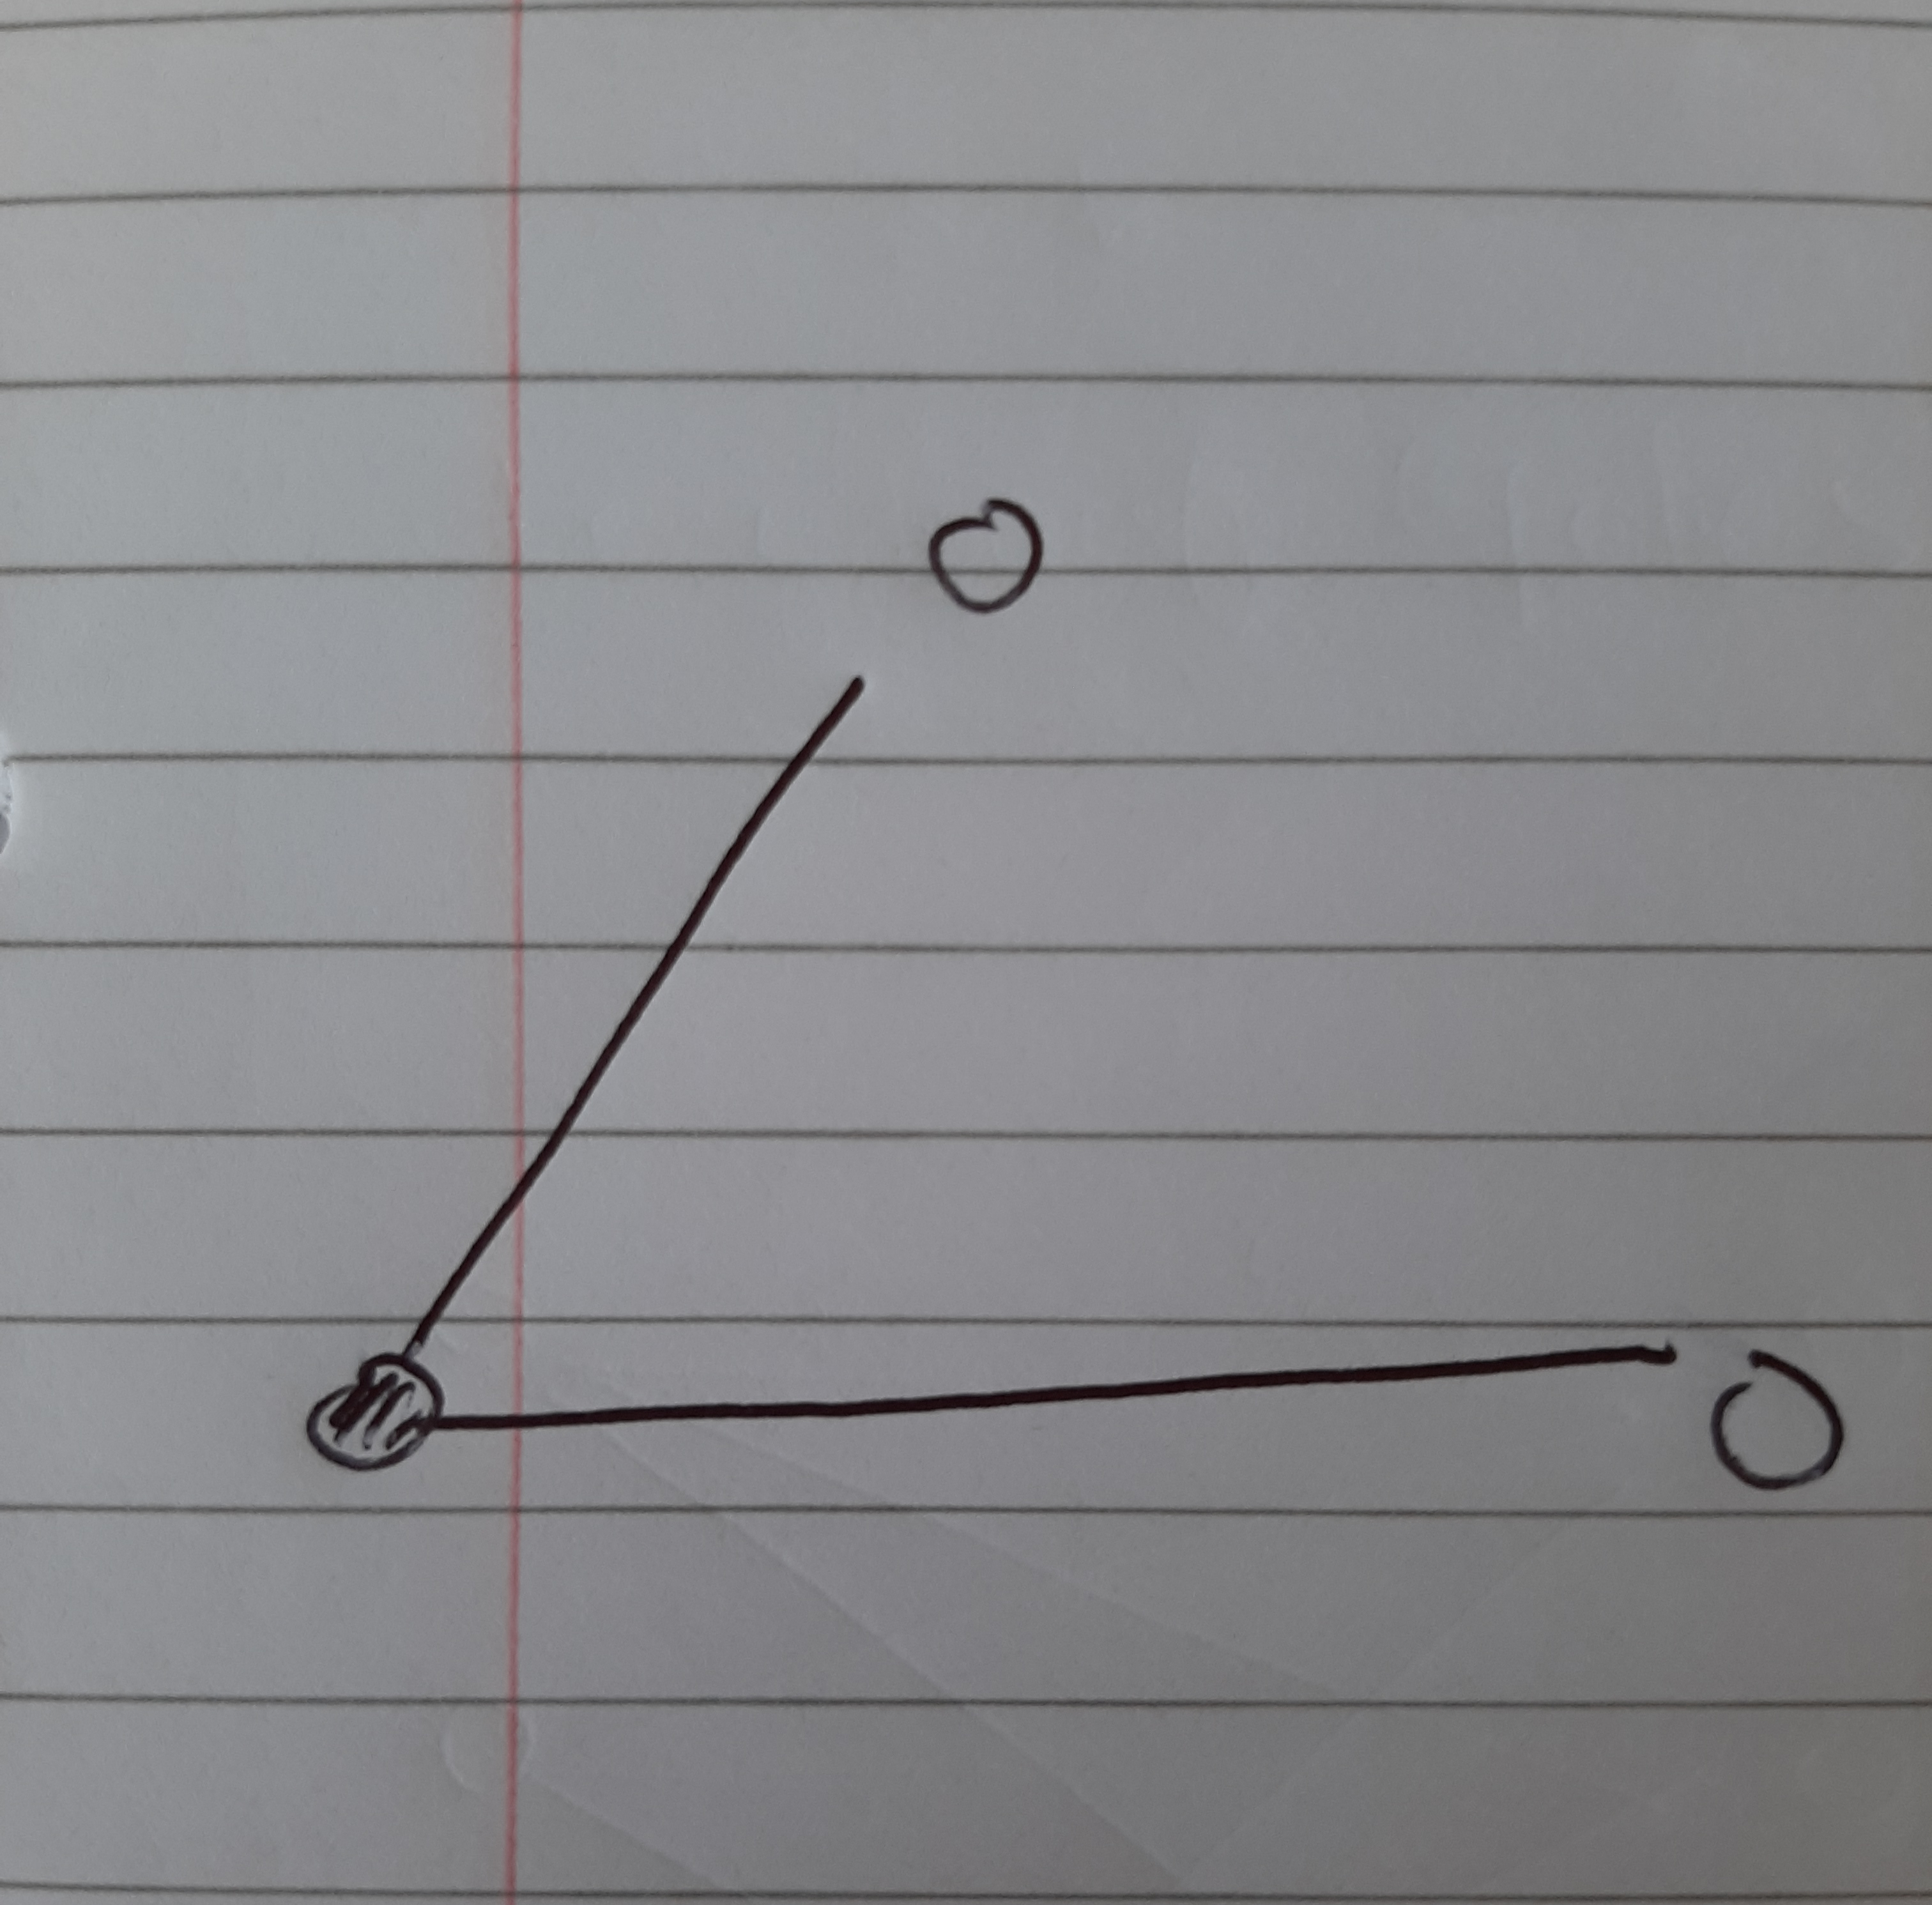
\includegraphics[width=0.4\linewidth]{images/worksheet_20_q1c_comments_1.jpg}
        % \end{center}

        \item Cycle with even number of verticies - Bipartite

        % \begin{center}
        % 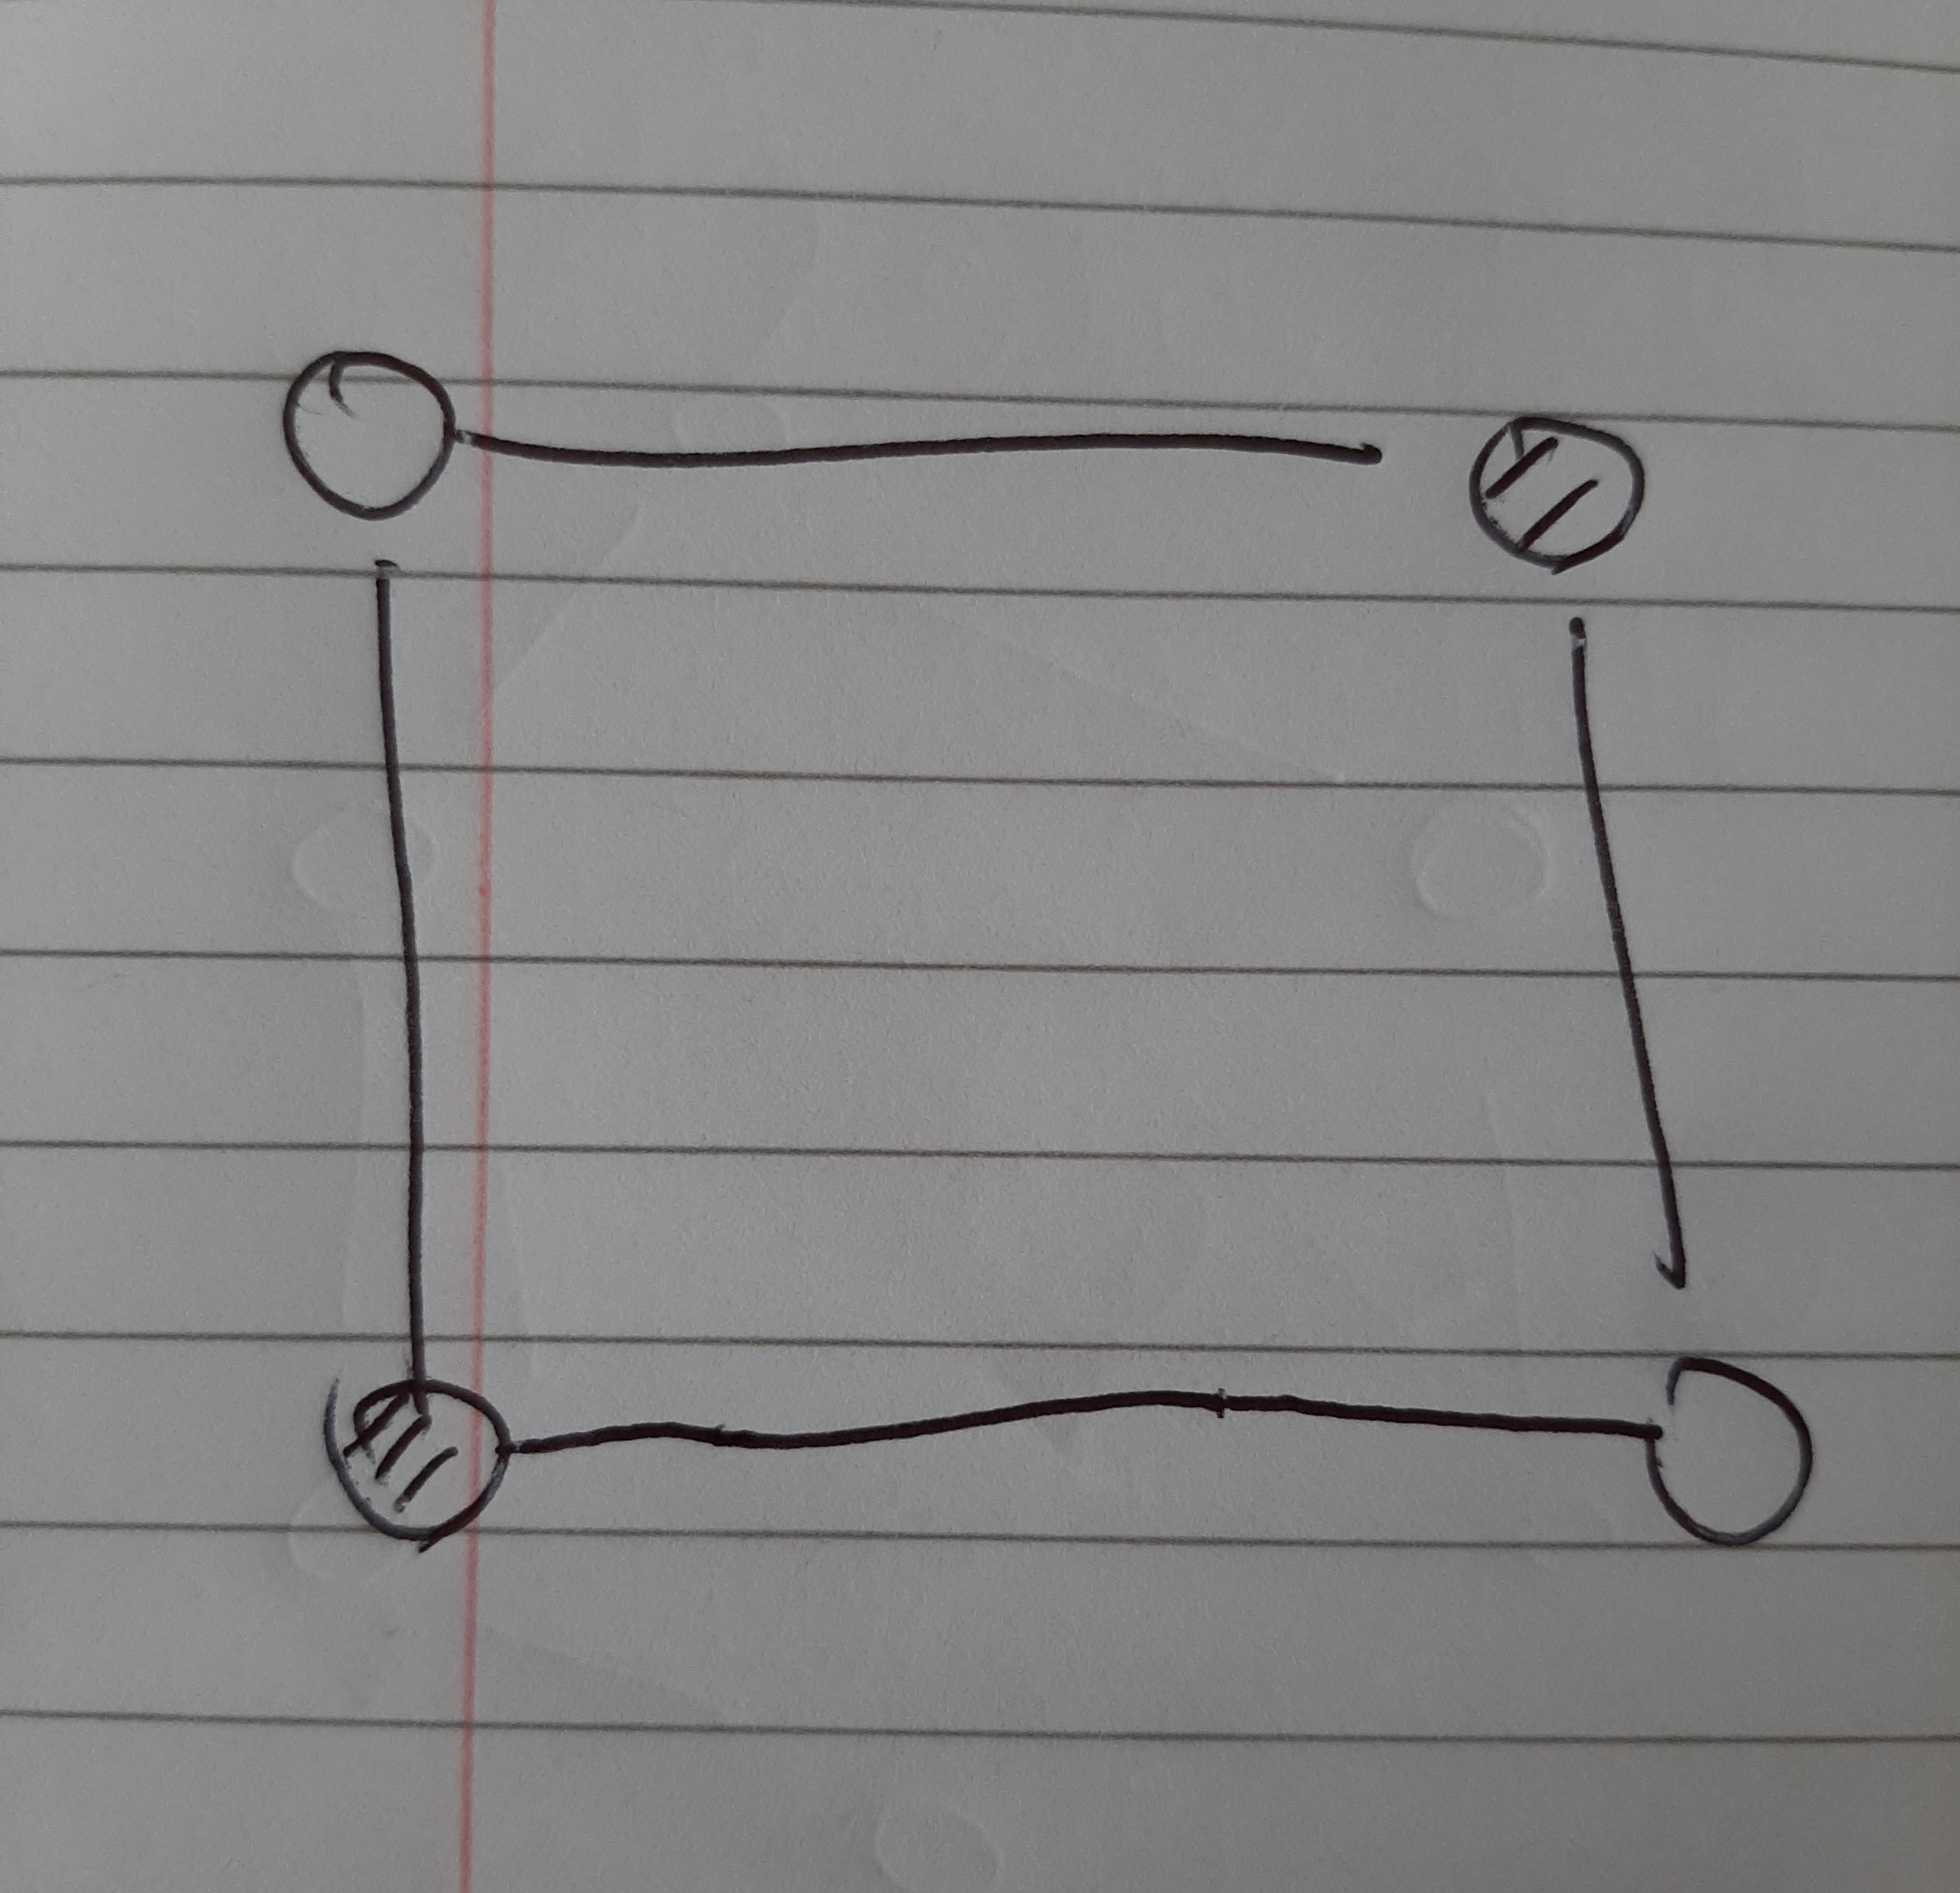
\includegraphics[width=0.4\linewidth]{images/worksheet_20_q1c_comment_2.jpg}
        % \end{center}

        \item 뚜퍼맨!! 영차! 영차! 형모 풀뚜있쪄!!
        \item 할뚜있다 형모야!!
        \item 형모 많이 틀렸쬬
        \item 형모 틀리면 틀리면서 배우면 되느니라. 흠허허허허!!
        \item 형모 화이팅!!
        \item 파이팅 파이팅!!
        \item 형모 해낼 수 있쬬!!!
        \item 형모야. 한걸음 더.
        \item 고마워요
        \item 여보, 사랑해요

    \end{itemize}

\end{enumerate}

\end{document}